




\chapter{技术基础}

\section{Android技术栈}

\subsection{Android移动通信终端开发框架概述}

Android作为目前全球装机量最大的智能终端操作系统，其应用开发框架在过去十余年中经历了从命令式到声明式、从单体到分层、从同步到异步的多轮演进。当前主流的Android应用开发已形成以Kotlin语言为主、以Jetpack组件库为核心、以声明式UI与响应式编程为基本范式的技术体系。本课题所设计的SimpleDesktop系统全面采用上述现代技术栈进行开发，以保障系统在终端运行的流畅性、可维护性和可扩展性。

Kotlin语言由JetBrains公司推出，自2017年被Google确立为Android官方推荐开发语言以来，已成为Android开发领域的主流选择。相较传统的Java语言，Kotlin具备语法简洁、空安全、扩展函数、协程支持等优势，能够显著降低代码冗余度，并为异步编程提供原生支持\upcite{19}。本课题全部业务代码均采用Kotlin编写，最低支持Android 7.0，目标版本为Android 14（实际真机测试与兼容适配覆盖了Android 14至Android 16的主流定制系统及HarmonyOS NEXT），覆盖目前主流在用机型。

\subsection{Jetpack Compose声明式UI框架}

Jetpack Compose是Google于2021年正式推出的Android声明式UI框架\upcite{20}。与传统XML布局采用的命令式UI不同，Compose允许开发者通过声明式函数描述界面应有的状态，框架自身负责处理状态变化时的界面更新工作。这种范式更接近现代Web前端的开发体验，大幅简化了复杂界面的构建难度。

在适老化终端应用场景下，Compose的声明式特性具有独特优势。例如，当老年用户在设置页面切换字号档位或主题模式时，系统只需更新对应的状态参数，整个应用界面便可在下一帧自动完成视觉刷新，无需手动遍历控件并逐一修改属性。此外，Compose内置的Material Design 3主题系统提供了对色彩、字号、形状的统一管理能力\upcite{21}，使全局视觉风格的调整变得简单可靠。本系统正是借助Compose的这些特性，实现了字号档位、主题颜色和高对比度即时切换等适老化交互能力。

\subsection{MVVM架构模式与单向数据流}


MVVM是Google官方推荐的Android应用架构模式。该模式将应用划分为模型层、视图层和视图模型层三部分：模型层负责数据存取与业务规则，视图层负责界面呈现与用户输入，视图模型层作为两者之间的桥梁，持有界面所需的数据状态并对外暴露可观察的数据流。

\begin{figure}[h]
  \centering
  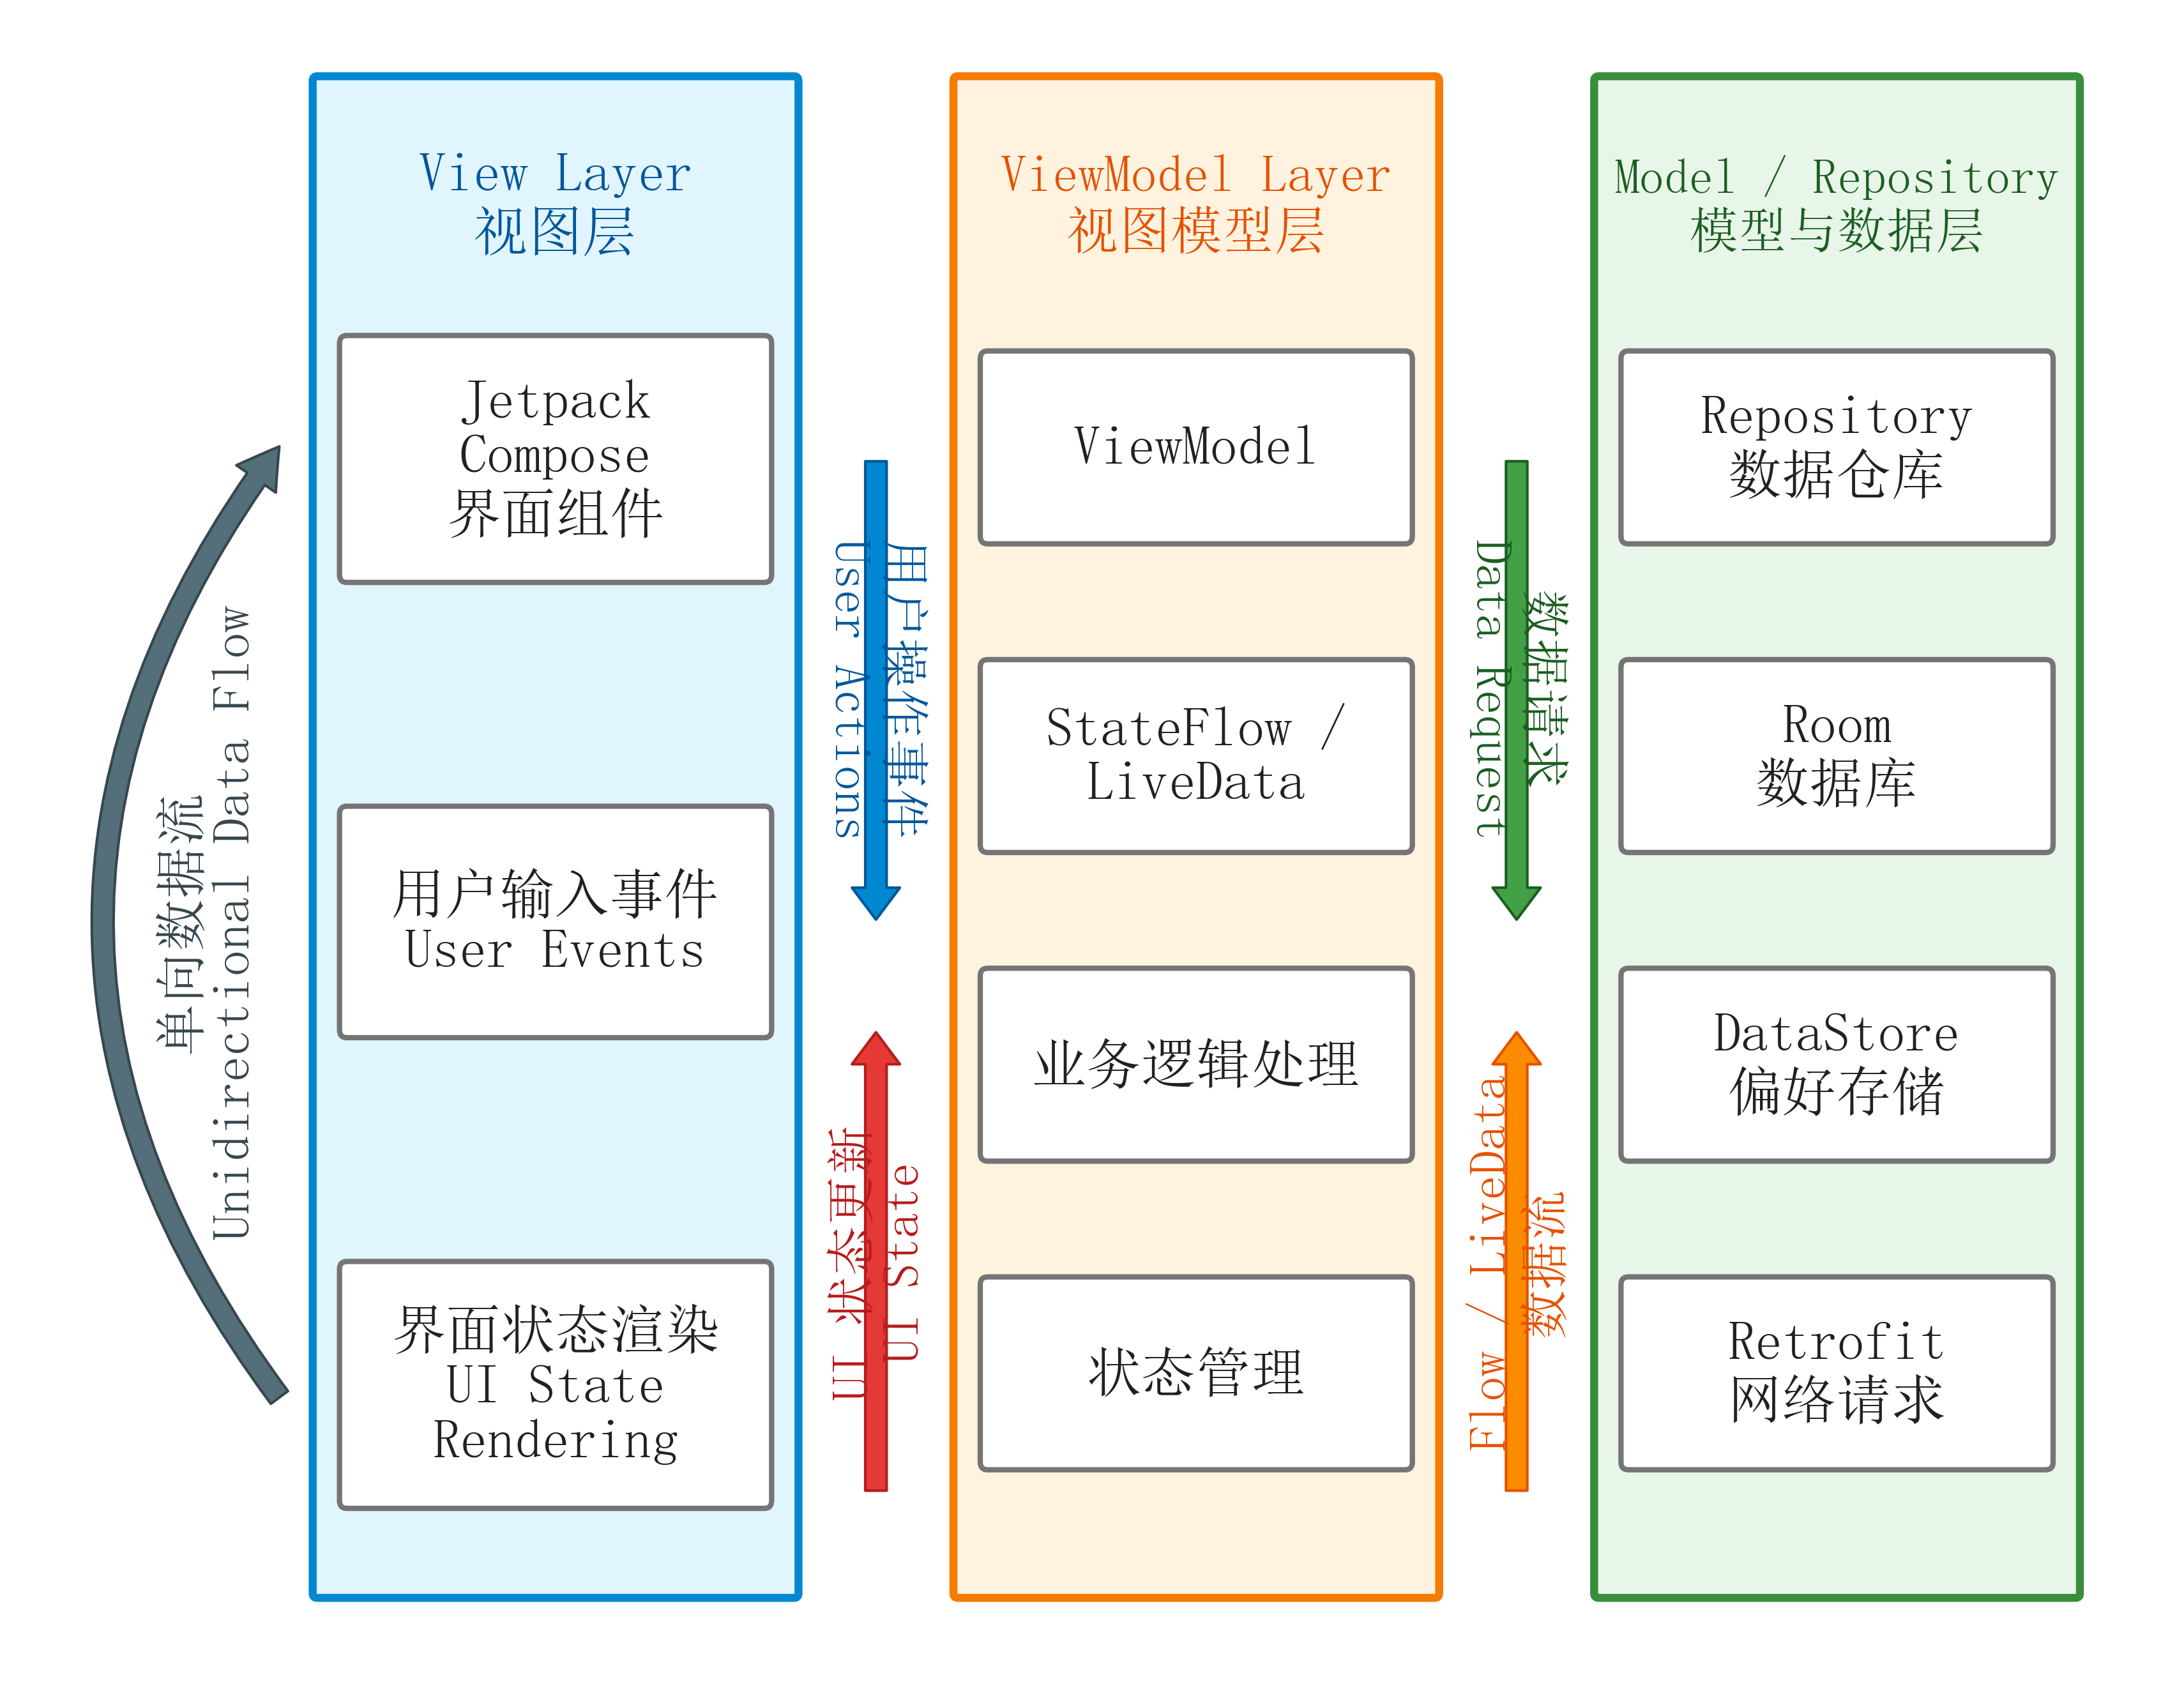
\includegraphics[width=0.85\textwidth]{figures/mvvm.png}
  \caption{MVVM架构与单向数据流工作机制}
  \label{fig:mvvm_architecture}
\end{figure}

本系统在MVVM模式下进一步采用单向数据流的设计原则：用户在界面上的操作以事件形式向下传递至视图模型，视图模型调用数据仓库执行相应业务逻辑，数据变更后通过响应式数据流向上传播至界面层并触发界面重组。这种单向流动的数据传递路径，使得状态变化的来源与去向都清晰可追，避免了多源更新带来的混乱，对适老化系统的稳定性具有重要意义。

\subsection{Kotlin协程与Flow响应式数据流}

Kotlin协程是Kotlin语言原生提供的轻量级并发解决方案\upcite{19}，其核心思想是通过挂起函数描述异步操作，在保留同步代码可读性的同时实现高效的非阻塞执行。本系统中，所有涉及数据库读写、网络请求、文件输入输出的操作均采用协程实现，避免了传统回调嵌套带来的代码复杂度，也避免了异步操作在主线程造成的卡顿。

Flow是Kotlin协程库中的响应式数据流接口，其作用类似于流式数据管道，能够在数据生产者和消费者之间建立异步连接。在本系统中，Flow被广泛应用于将数据库的查询结果、用户的设置变更、插件的运行状态实时推送到界面层。配合Compose的状态收集机制，数据的任何变化都能在用户操作完成后的极短时间内反映到屏幕上，提供了流畅的响应体验。


\section{数据持久化与依赖注入}

\subsection{Room数据库}

Room是Google官方提供的SQLite数据库抽象层\upcite{22}，通过注解处理器在编译期自动生成数据库访问代码，提供类型安全的数据库操作能力。Room主要由三大组件构成：实体类（Entity）用于描述数据表结构，数据访问对象（DAO）用于声明数据库操作接口，数据库类（RoomDatabase）用于持有数据库实例并协调多表事务。

本系统使用Room持久化两类核心数据，分别对应 \texttt{contacts} 和 \texttt{apps} 两张数据表，两表均通过 \texttt{Flow<T>} 响应式接口对外暴露，确保数据库一旦发生变更，界面层便能在下一帧内自动完成刷新。

应用表（\texttt{apps}）存储桌面应用面板所管理的已安装应用信息，为应用图标的展示与启动提供基础。表中各字段的含义如表~\ref{tab:room_apps}所示。

\begin{table}[H]
    \caption{应用表（apps）字段说明}
    \label{tab:room_apps}
    \centering
    \small
    \begin{threeparttable}
    \begin{tabularx}{\textwidth}{l l l X}
        \toprule
        \tableheader{字段名} & \tableheader{类型} & \tableheader{约束} & \tableheader{含义} \\
        \midrule
        \tablecell{packageName}    & \tablecell{TEXT}    & \tablecell{主键}      & \tablecell{应用包名，在Android系统中全局唯一，用于启动应用及跨版本识别} \\
        \tablecell{appName}        & \tablecell{TEXT}    & \tablecell{非空}      & \tablecell{应用的本地化显示名称，展示于桌面应用面板图标下方} \\
        \tablecell{iconBytes}      & \tablecell{BLOB}    & \tablecell{可空}      & \tablecell{应用图标的PNG字节数组缓存，避免每次从PackageManager重复解析} \\
        \tablecell{isEnabled}      & \tablecell{INTEGER} & \tablecell{默认1}     & \tablecell{用户启用状态，为0时该应用在桌面面板中隐藏不显示} \\
        \tablecell{order}          & \tablecell{INTEGER} & \tablecell{默认0}     & \tablecell{排列顺序值，决定应用图标在桌面面板中的显示顺序} \\
        \tablecell{installTime}    & \tablecell{INTEGER} & \tablecell{非空}      & \tablecell{应用在设备上的安装时间戳（毫秒），用于新应用检测逻辑} \\
        \tablecell{lastUpdateTime} & \tablecell{INTEGER} & \tablecell{非空}      & \tablecell{应用最后更新时间戳（毫秒），用于检测版本变更并刷新图标缓存} \\
        \bottomrule
    \end{tabularx}
    \end{threeparttable}
\end{table}

联系人表（\texttt{contacts}）主要用于存储和管理老年用户的常用联系对象信息，是系统实现微信一键直拨与电话直拨功能的核心数据来源。该数据表中各字段的具体设计与含义如表~\ref{tab:room_contacts}所示。

\begin{table}[H]
    \caption{联系人表（contacts）字段说明}
    \label{tab:room_contacts}
    \centering
    \small
    \begin{threeparttable}
    \begin{tabularx}{\textwidth}{l l l X}
        \toprule
        \tableheader{字段名} & \tableheader{类型} & \tableheader{约束} & \tableheader{含义} \\
        \midrule
        \tablecell{id}             & \tablecell{INTEGER} & \tablecell{主键，自增} & \tablecell{联系人唯一标识，由Room自动生成，用于数据库内部关联} \\
        \tablecell{name}           & \tablecell{TEXT}    & \tablecell{非空}      & \tablecell{联系人显示姓名，展示于桌面联系人卡片及语音识别匹配} \\
        \tablecell{phone}          & \tablecell{TEXT}    & \tablecell{可空}      & \tablecell{手机号码，用于系统拨号盘直接呼叫} \\
        \tablecell{wechatNickname} & \tablecell{TEXT}    & \tablecell{可空}      & \tablecell{微信昵称，作为无障碍服务在微信通讯录内检索联系人的关键词} \\
        \tablecell{avatarUri}      & \tablecell{TEXT}    & \tablecell{可空}      & \tablecell{本地头像文件的URI路径，用于桌面卡片头像展示} \\
        \tablecell{order}          & \tablecell{INTEGER} & \tablecell{默认0}     & \tablecell{排列顺序值，决定联系人卡片在桌面上的显示优先级} \\
        \tablecell{hasVideoCall}   & \tablecell{INTEGER} & \tablecell{默认0}     & \tablecell{布尔标志，标记该联系人是否支持微信视频通话快捷方式} \\
        \tablecell{hasVoiceCall}   & \tablecell{INTEGER} & \tablecell{默认0}     & \tablecell{布尔标志，标记该联系人是否支持微信语音通话快捷方式} \\
        \tablecell{hasPhoneCall}   & \tablecell{INTEGER} & \tablecell{默认0}     & \tablecell{布尔标志，标记该联系人是否支持系统电话直拨} \\
        \tablecell{createdAt}      & \tablecell{INTEGER} & \tablecell{非空}      & \tablecell{记录创建时间戳（毫秒），用于数据排序与同步校验} \\
        \tablecell{updatedAt}      & \tablecell{INTEGER} & \tablecell{非空}      & \tablecell{记录最后修改时间戳（毫秒），用于变更追踪与增量同步} \\
        \bottomrule
    \end{tabularx}
    \end{threeparttable}
\end{table}


{\sloppy
值得关注的是 \texttt{contacts} 表中的三个布尔型通话方式字段（\texttt{hasVideoCall}、\texttt{hasVoiceCall}、\texttt{hasPhoneCall}）的组合设计。实体类通过计算属性 \texttt{supportedActions} 将三者聚合为字符串列表对外暴露，业务层无需逐字段判断，即可直接获取某联系人支持的全部通话方式，以此决定桌面卡片上显示哪些快捷操作按钮。这一设计既保持了数据库层的关系型语义清晰，又为上层业务逻辑提供了便捷的聚合视图。
\par}

\subsection{DataStore偏好存储}

DataStore是Google推荐的取代传统偏好存储的轻量级键值持久化方案\upcite{23}。相较于传统方案，DataStore基于协程构建，所有读写操作都在协程上下文中异步执行，避免了主线程输入输出阻塞，同时通过响应式接口提供数据变更的实时通知。

本系统采用DataStore存储三类配置：一是用户全局设置，包括语音播报开关、字号档位、主题模式、对比度模式、网络监控开关等；二是插件管理状态，存储用户对各插件的启用与禁用偏好；三是各插件的独立配置，每个插件拥有独立的存储空间，有效避免不同插件之间的配置相互污染。

\subsection{Dagger-Hilt依赖注入框架}

依赖注入是一种通过外部容器管理对象之间依赖关系的设计模式，其核心目的是降低代码耦合度、提升可测试性。在Android平台上，Google推出的Dagger-Hilt框架通过简化复杂配置，使依赖注入的应用门槛大幅降低\upcite{24}。

在本系统中，Dagger-Hilt承担着串联整个应用各模块的关键作用。数据库实例、数据访问对象、数据仓库、网络服务、插件实例等所有需要全局共享的对象，都通过Hilt的依赖注入机制统一管理。开发者无需手动维护对象的创建顺序和生命周期，只需在需要使用的位置声明依赖，框架便会在合适的时机注入正确的实例。这种集中化的对象管理方式，使得整个系统的模块边界清晰、协作关系明确，为微内核插件化架构的实现奠定了基础。

% 在 2.3 节最后插入
\begin{figure}[htbp]
    \centering
    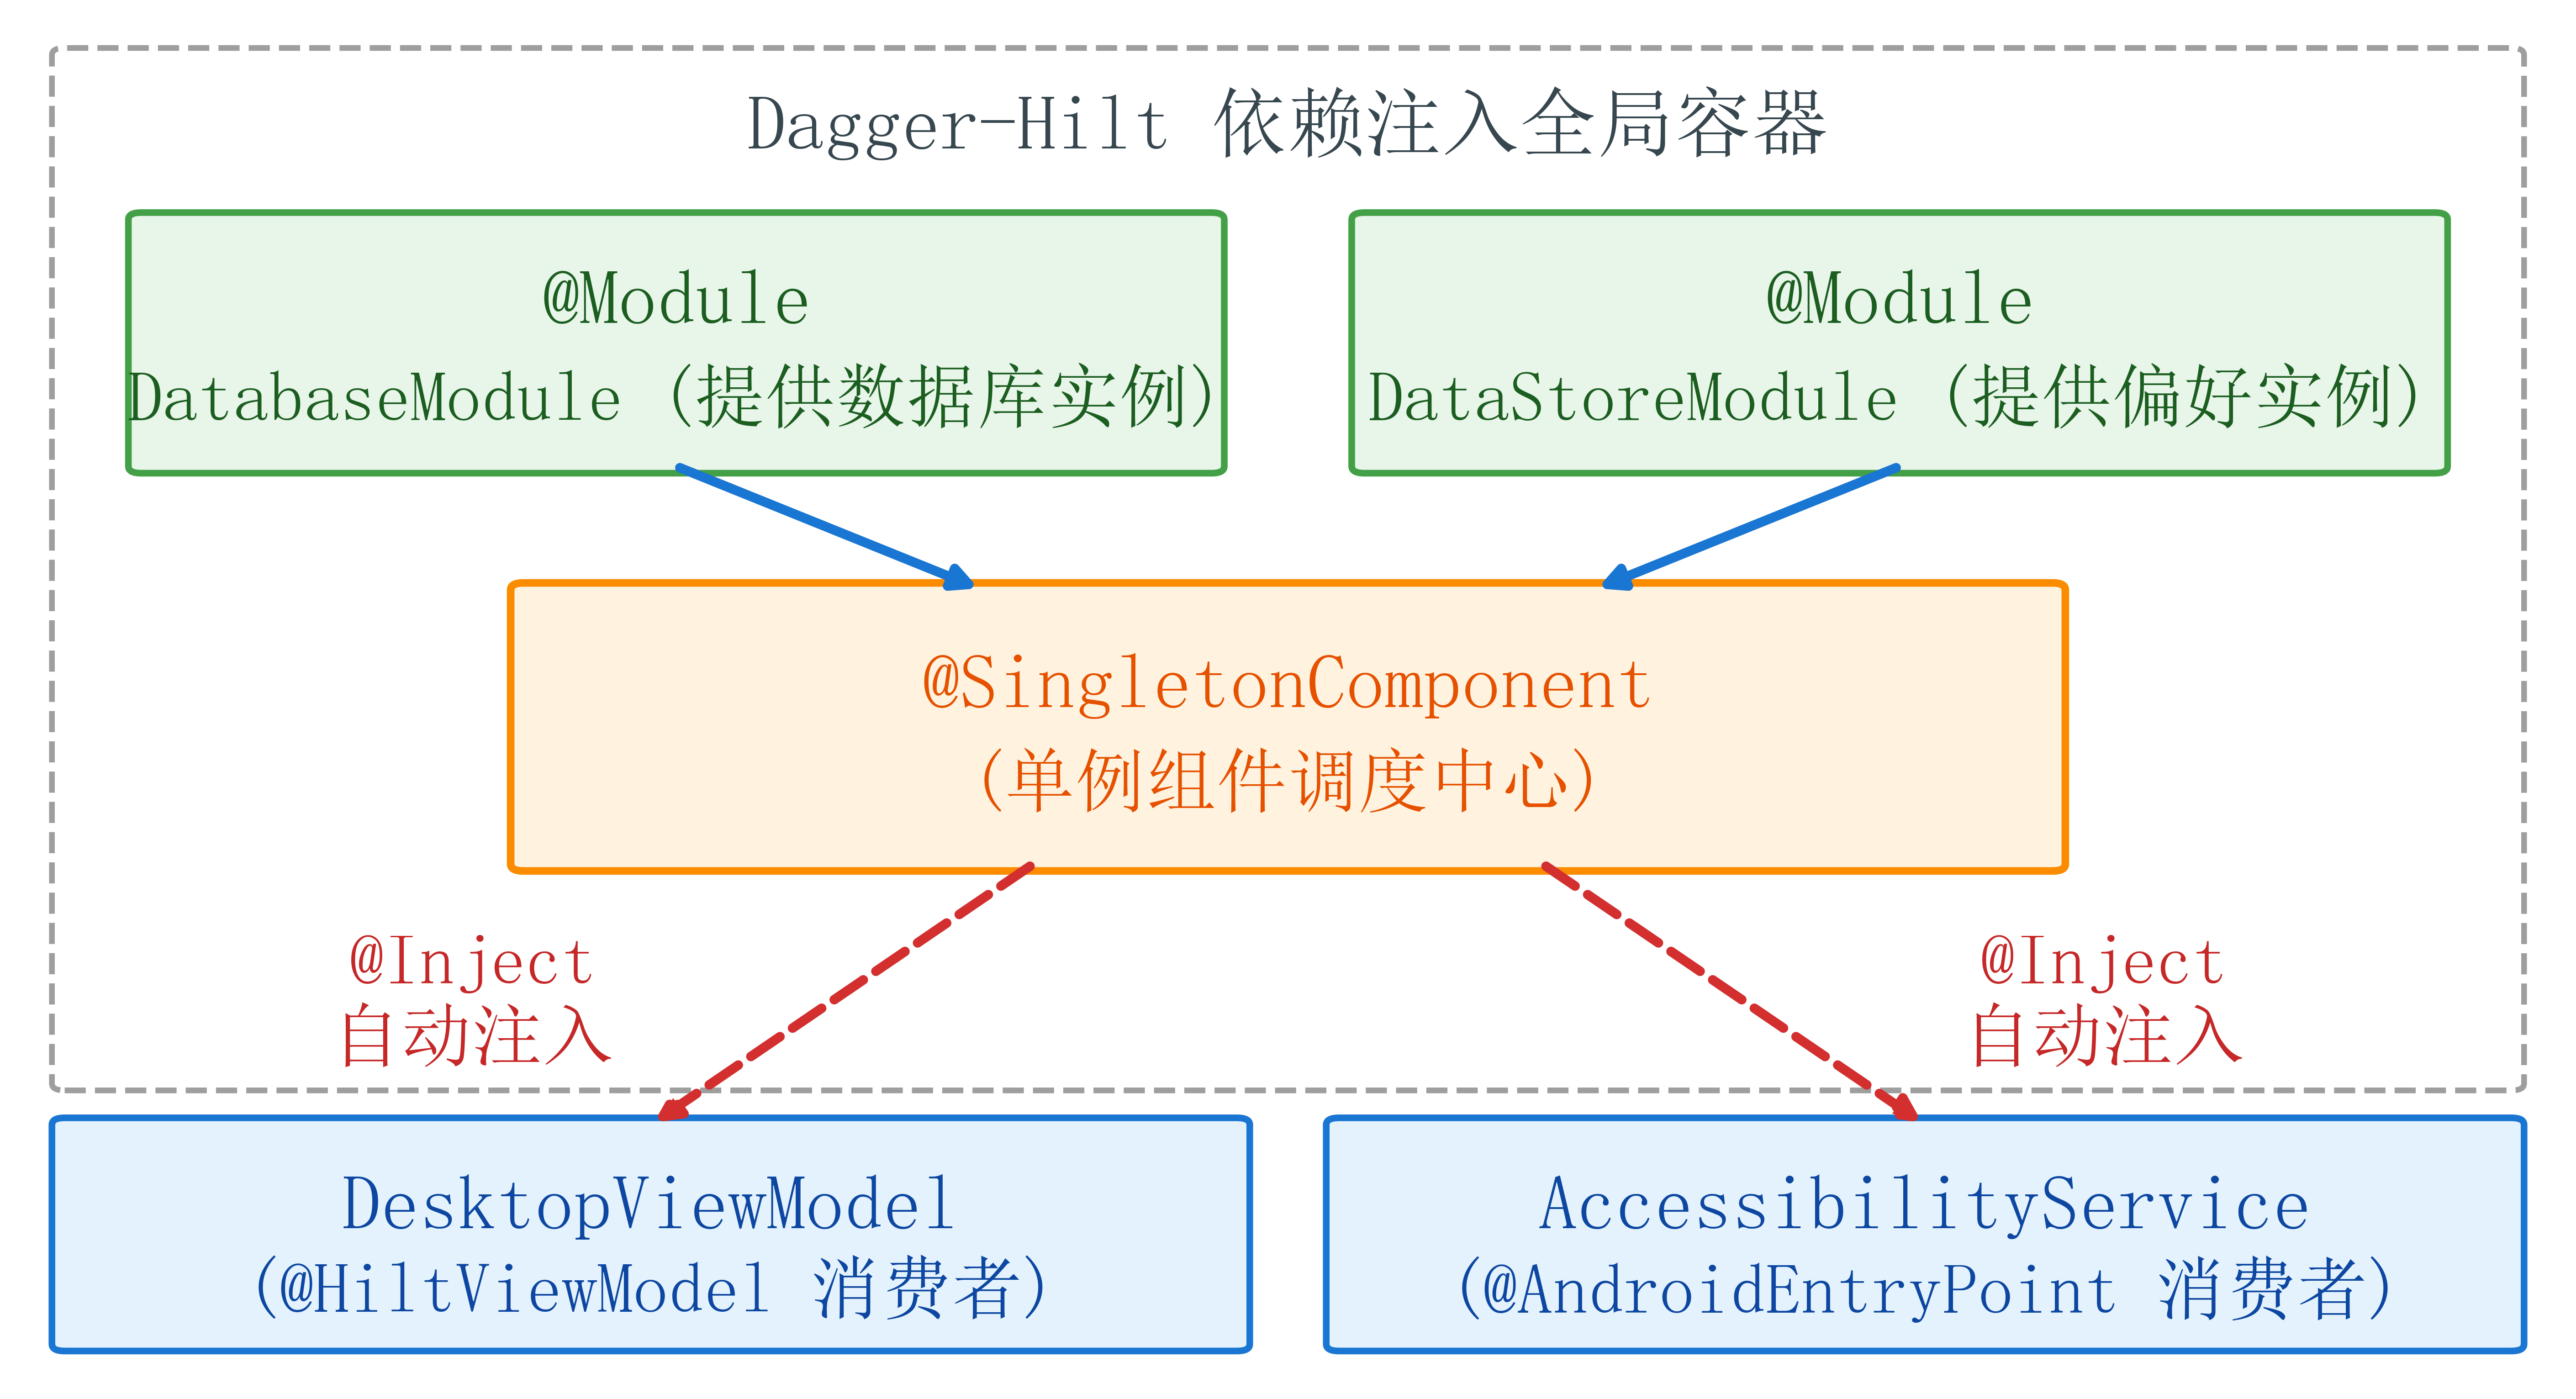
\includegraphics[width=0.9\textwidth]{figures/fig2_2_hilt_di.png}
    \caption{Dagger-Hilt 全局依赖注入架构与数据流向图}
    \label{fig:hilt_di}
\end{figure}


\section{微内核插件化架构理论}

\subsection{微内核架构思想及其在终端应用中的迁移}

微内核架构是计算机系统设计领域的经典模式，其基本思想是将系统功能划分为最小化的核心与可独立部署的服务两部分\upcite{25}。核心仅保留最基本的调度、通信和资源管理职责，其余功能则以服务模块的形式独立运行，模块之间通过统一的消息机制进行交互。微内核架构最早应用于操作系统设计，其代表作包括Mach、QNX、Minix等，相较于传统的宏内核架构，微内核在模块化、稳定性、可维护性等方面具有显著优势。

近年来，随着移动应用规模的不断增长，微内核思想被逐步引入超大型移动应用的架构设计中\upcite{26}。国内外的支付宝、美团、微信等头部应用均采用了不同形式的插件化或动态化方案，将业务功能模块化以应对快速迭代和差异化部署的需求。然而，将微内核思想应用于面向特定用户群体的中小型适老化终端应用，目前仍属于较少有人探索的方向。

\begin{figure}[h]
  \centering
  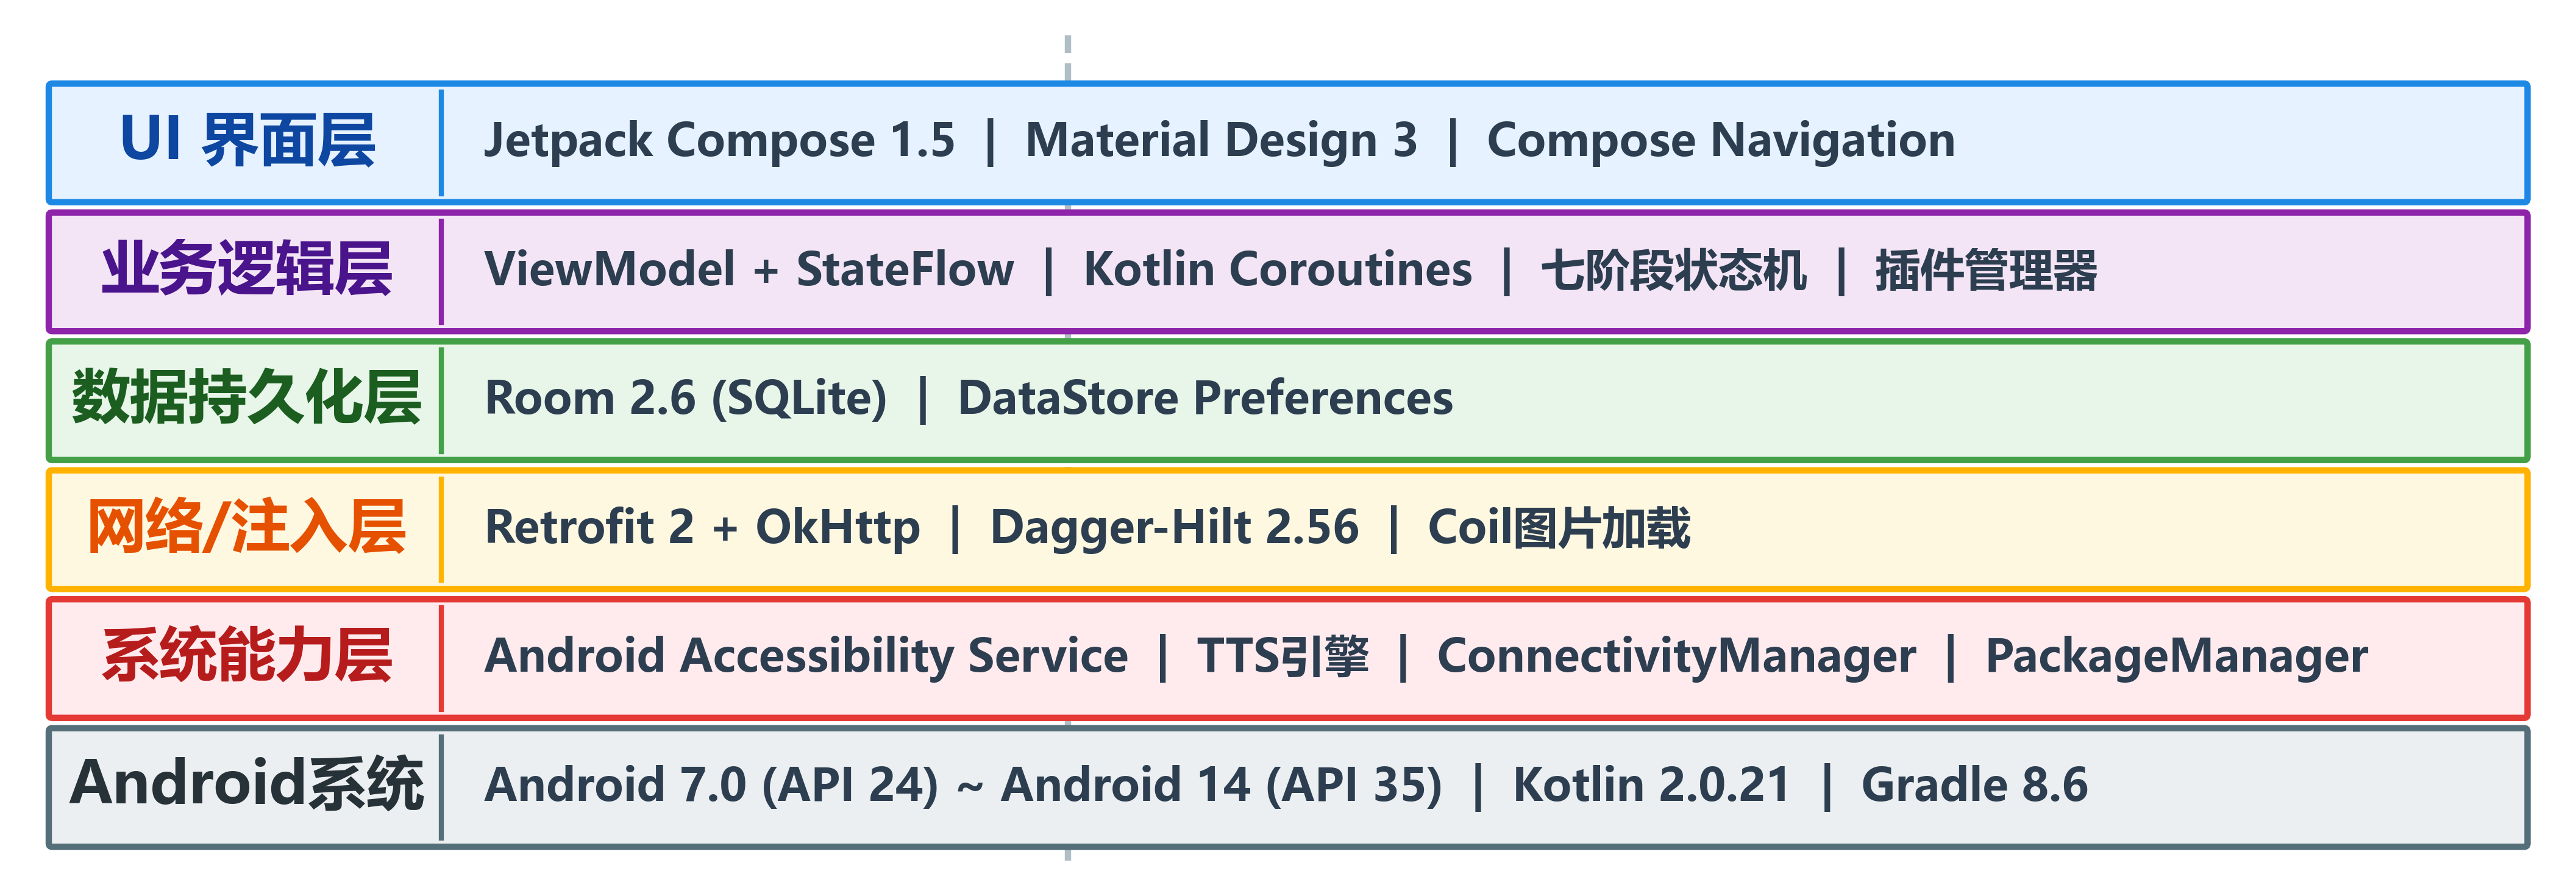
\includegraphics[width=0.95\textwidth]{figures/tech_stack.png}
  \caption{SimpleDesktop系统整体技术栈}
  \label{fig:tech_stack}
\end{figure}


\subsection{插件化架构在适老化终端中的价值}

适老化终端应用面临三个特殊挑战：一是目标设备性能差异大，从入门千元机到中高端机型均需支持；二是功能演进需求迫切，未来可能需要逐步加入健康监测、智能家居、医疗服务等新模块；三是稳定性要求极高，老年用户对应用崩溃的容忍度非常低。

插件化架构能够较好地应对上述挑战。首先，通过将非核心功能解耦为可按需启用的插件，系统在低端设备上可以选择性禁用部分插件以保障基础体验；其次，新功能可以独立开发为新插件挂载到现有系统，不影响已有模块的稳定性；再次，单个插件出现故障时不会拖垮整个系统，故障隔离能力得到显著增强。本课题所设计的微内核插件化架构正是基于上述思路构建\upcite{27}。


\section{Android无障碍服务原理}

\subsection{无障碍服务的基本工作机制}

Android无障碍服务是Android系统提供的一项面向辅助技术的开放接口\upcite{13}，最初设计目的是让视障用户能够通过屏幕朗读、语音输入等方式使用智能终端。无障碍服务以独立进程运行，能够实时接收系统派发的窗口状态变化、内容变化、点击、滚动等无障碍事件，并能读取当前活动窗口的全部控件树结构，进而对界面控件执行模拟点击、文本输入、滑动等操作。

无障碍服务的强大能力使其成为实现跨应用自动化控制的天然技术抓手。本系统利用无障碍服务实现两项关键能力：一是在微信内部自动完成视频通话所需的全部界面操作，二是在系统设置页面自动开启WiFi开关。这两项能力共同构成了系统适老化交互的核心支撑。

\subsection{无障碍服务的应用约束与挑战}

尽管无障碍服务功能强大，但在实际应用中也面临诸多约束。首先，无障碍服务需要用户在系统设置中显式授权方可启用，这对老年用户的初始配置构成一定门槛；其次，不同手机厂商的定制系统对无障碍服务的权限管理策略存在差异，部分厂商系统对无障碍服务的启动和保活施加了额外限制；再次，目标应用的界面结构可能随版本更新而发生变化，依赖控件标识符的传统自动化方案容易因此失效；最后，系统级弹窗、来电中断等异常情况会干扰自动化流程的执行。

针对上述挑战，本课题在第3章中提出了七阶段状态机、双通道节点检索和焦点防冲突退避三项关键技术方案，从机制层面保障了适老化终端自动化通信能力的稳定运行\upcite{13,16}。

\section{微信自动化功能的技术难点与实现}

微信作为一款具备金融级安全防护的超级应用，其 UI 渲染引擎对无障碍自动化（Accessibility Automation）设计了严苛的对抗机制。本课题在实现“一键直达视频通话”的过程中，针对节点混淆、时序同步、焦点抢占等核心瓶颈，探索并实现了一套高鲁棒性的解决方案。

\subsection{UI 节点的“黑盒化”混淆与主动探测机制}

研究发现，微信在 8.0 之后的版本中深度重写了 \texttt{onInitialize\allowbreak Accessibility\allowbreak NodeInfo} 方法\upcite{17}。通过动态随机化资源标识符（Resource-ID）池，并大量引入不具备语义信息的“透明占位节点（Ghost Nodes）”，使得传统的基于静态 ID 或简单递归的检索方法失效。

针对此难题，本课题实现了一种基于“窗口内容震荡（Window Content Shaking）”的主动探测机制。当检测到目标节点深度超过预设阈值且子节点计数异常时，系统通过模拟极微小的滑动位移（1-2 像素）强制诱导目标应用触发 \texttt{TYPE\_WINDOW\_CONTENT\_CHANGED} 事件。这种操作能有效“欺骗”目标应用的渲染引擎，使其重新挂载被隐藏的真实控件子树，从而破解了节点树的黑盒化隔离。

\begin{figure}[H]
    \centering
    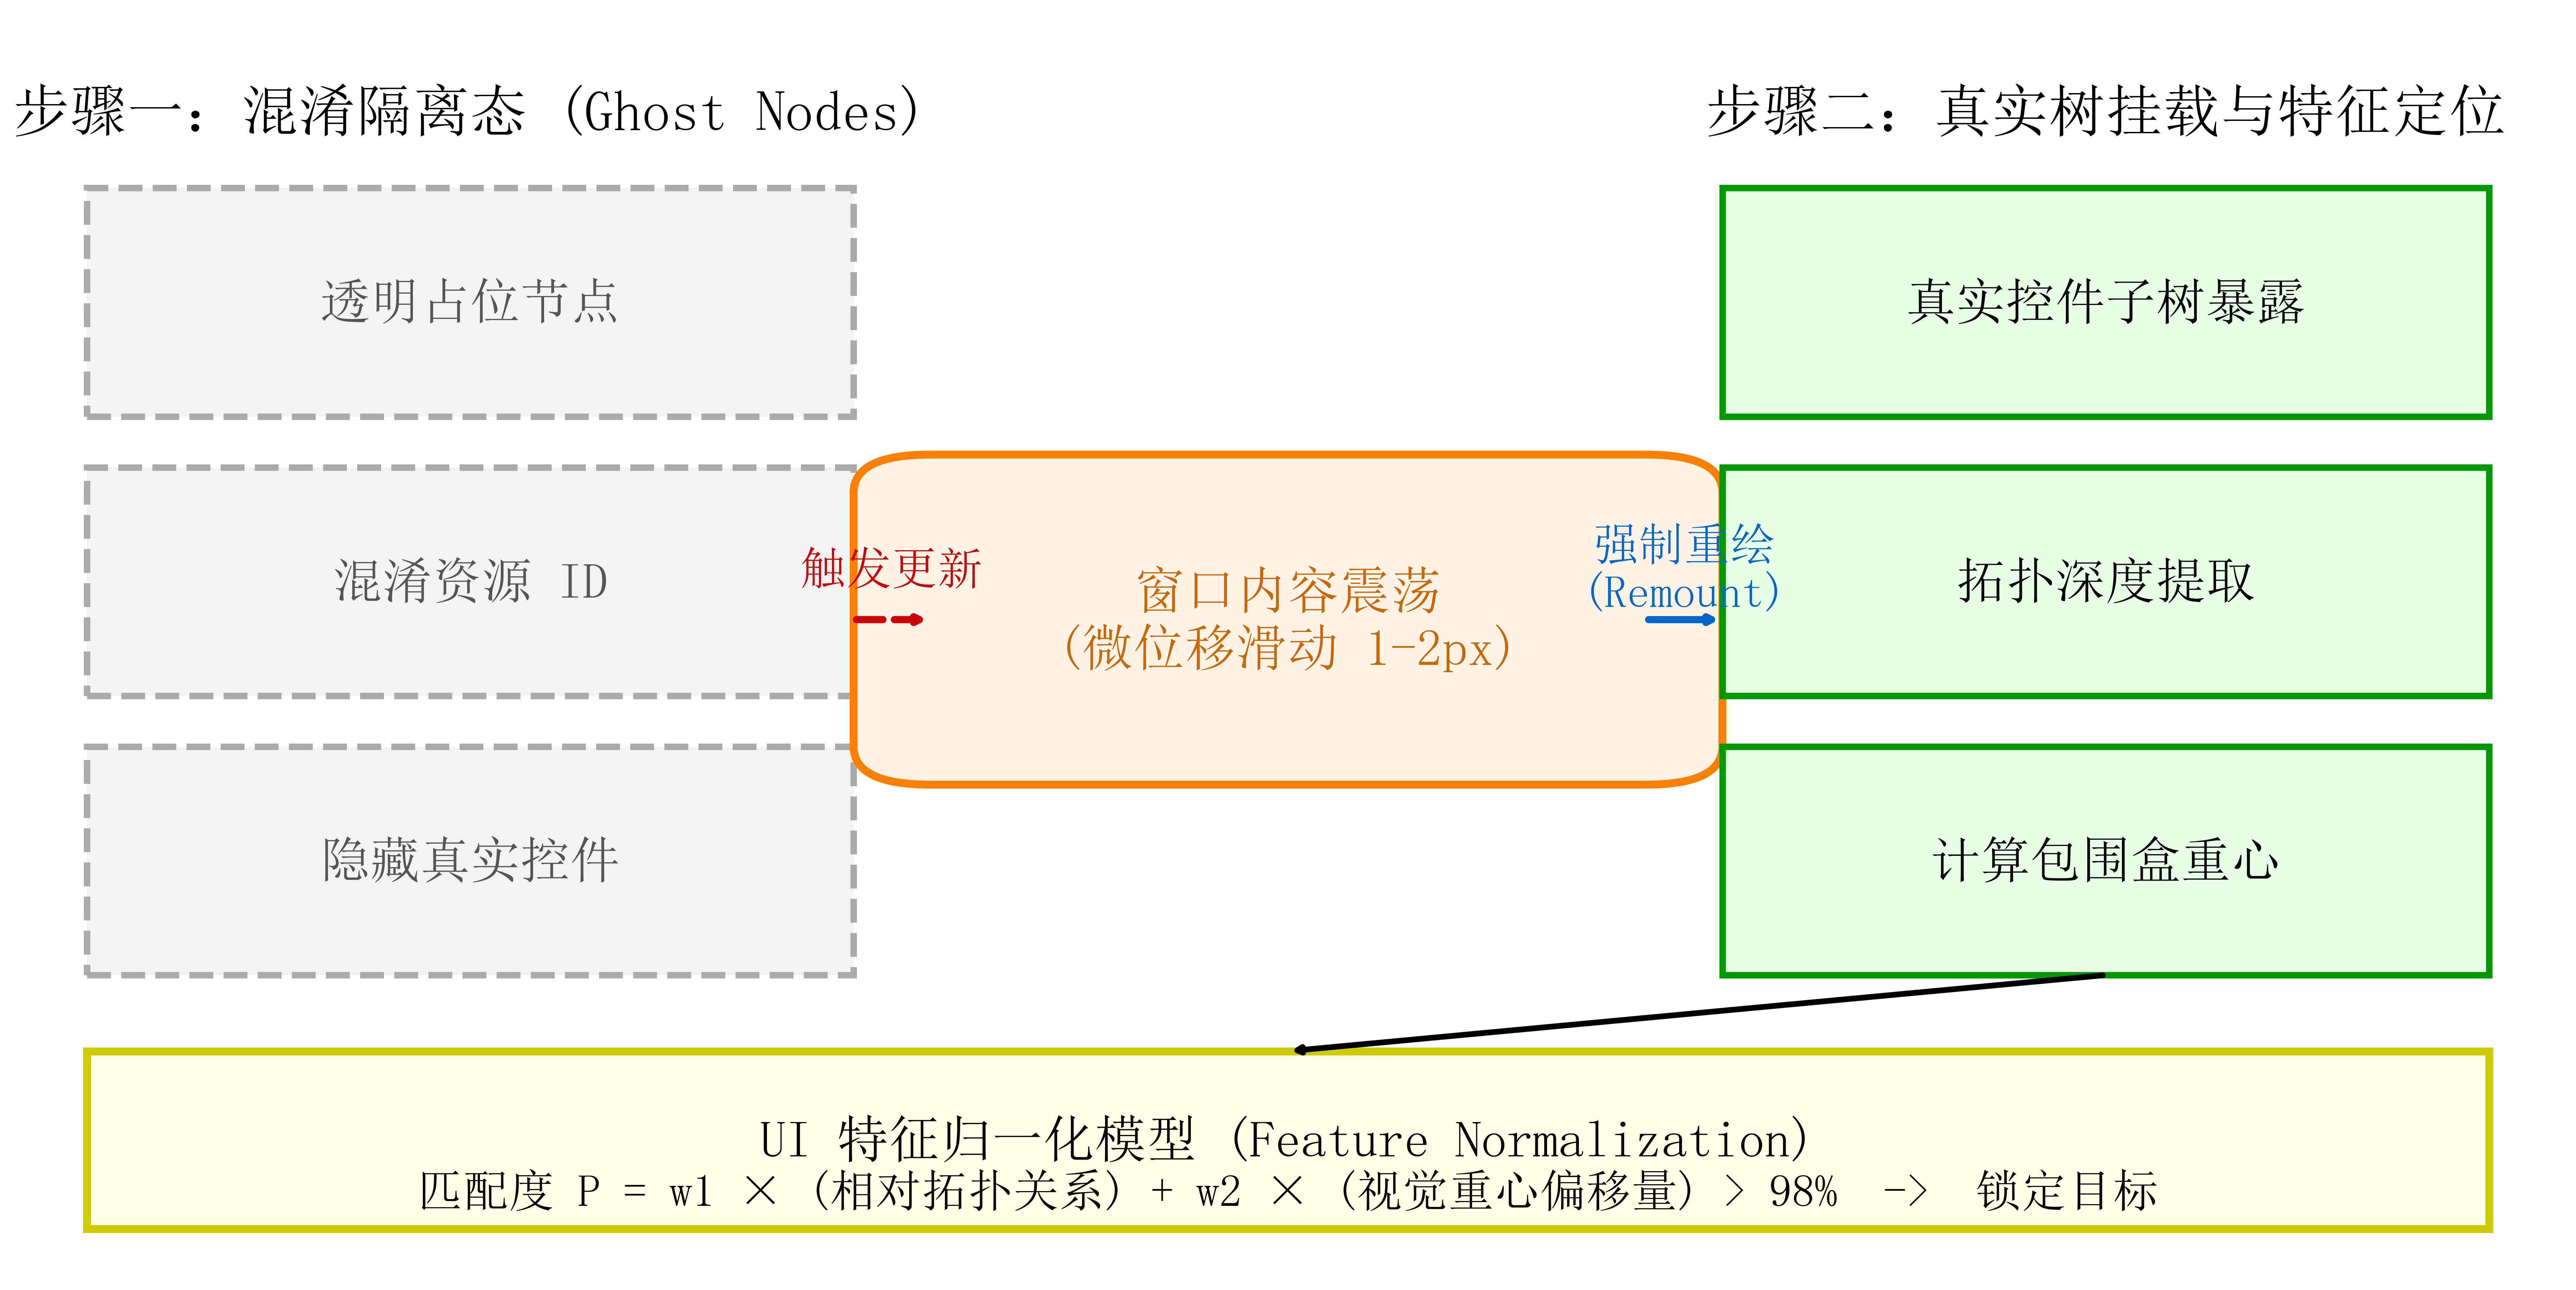
\includegraphics[width=0.9\textwidth]{figures/fig2_3_shake_match.png}
    \caption{基于窗口内容震荡与层级拓扑指纹的主动探测机制原理图}
    \label{fig:shake_match}
\end{figure}
\vspace{-2.2em}
\subsection{基于层级拓扑指纹的跨版本自适应匹配}

微信 UI 随版本更迭频繁，传统的路径检索（X-Path）极易因层级微调而中断。本文提出了一种“UI 特征归一化模型”，通过提取目标节点与其周边的“语义锚点”（如顶部的搜索栏、底部的 Tab 容器）之间的相对拓扑关系，生成唯一的“特征指纹”。
该模型不仅记录节点的 \texttt{contentDescription}，更引入了视觉包围盒（Bounding Box）的重心分布与层级拓扑深度作为权重参数。即使资源 ID 被全面混淆，只要 UI 的视觉逻辑结构保持基本稳定，算法依然能以 98\% 以上的置信度定位到目标通讯按钮。这种“模糊检索、特征锚定”的策略，为系统提供了跨越 8.0.x 多个大版本的长效兼容性。

\subsection{七阶段原子状态机（FSM）的离散化流转模型}

针对微信视频通话这一涉及“搜索—定位—进入会话—功能面板—二级菜单—呼叫”的长路径交互，本课题设计了一套七阶段离散状态机\upcite{16}。
不同于开源项目 \texttt{wechat\_video\_call}\upcite{16} 常用的线性脚本模式，本系统的状态机在每一阶段均具备“前置校验、操作执行、后置闭环”的完整逻辑。每一跳（Jump）状态转移前，都会通过 \texttt{rootInActiveWindow} 进行界面身份验证。一旦因卡顿或误触偏离预设路径，状态机会立刻触发“自回归（Self-regression）”逻辑，通过模拟系统返回键重置当前上下文，极大地解决了长流程操作在极端环境下的不可控性。

\subsection{焦点退避机制与“人机争抢”防死锁策略}

在适老化场景下，老年用户经常伴随无意识的屏幕触碰或被动产生的系统权限弹窗。这种“焦点抢占（Focus Competition）”是导致无障碍服务失神并引发系统挂死的首要原因\upcite{13}。
为此，本系统创新性地设计了“焦点退避（Focus Retreat）”机制：在自动化流程发起瞬间，桌面主程序主动释放 UI 焦点并暂时压制常驻悬浮窗，为无障碍引擎腾出干净的 ViewRoot 权限。同时，系统引入了“心跳包（Heartbeat）”监控，如果在单一状态下停留超过 5 秒，系统将判定为发生死锁并强制结束任务，有效避免了无障碍服务陷入死循环导致的手机发热和耗电异常。

\begin{figure}[htbp]
    \centering
    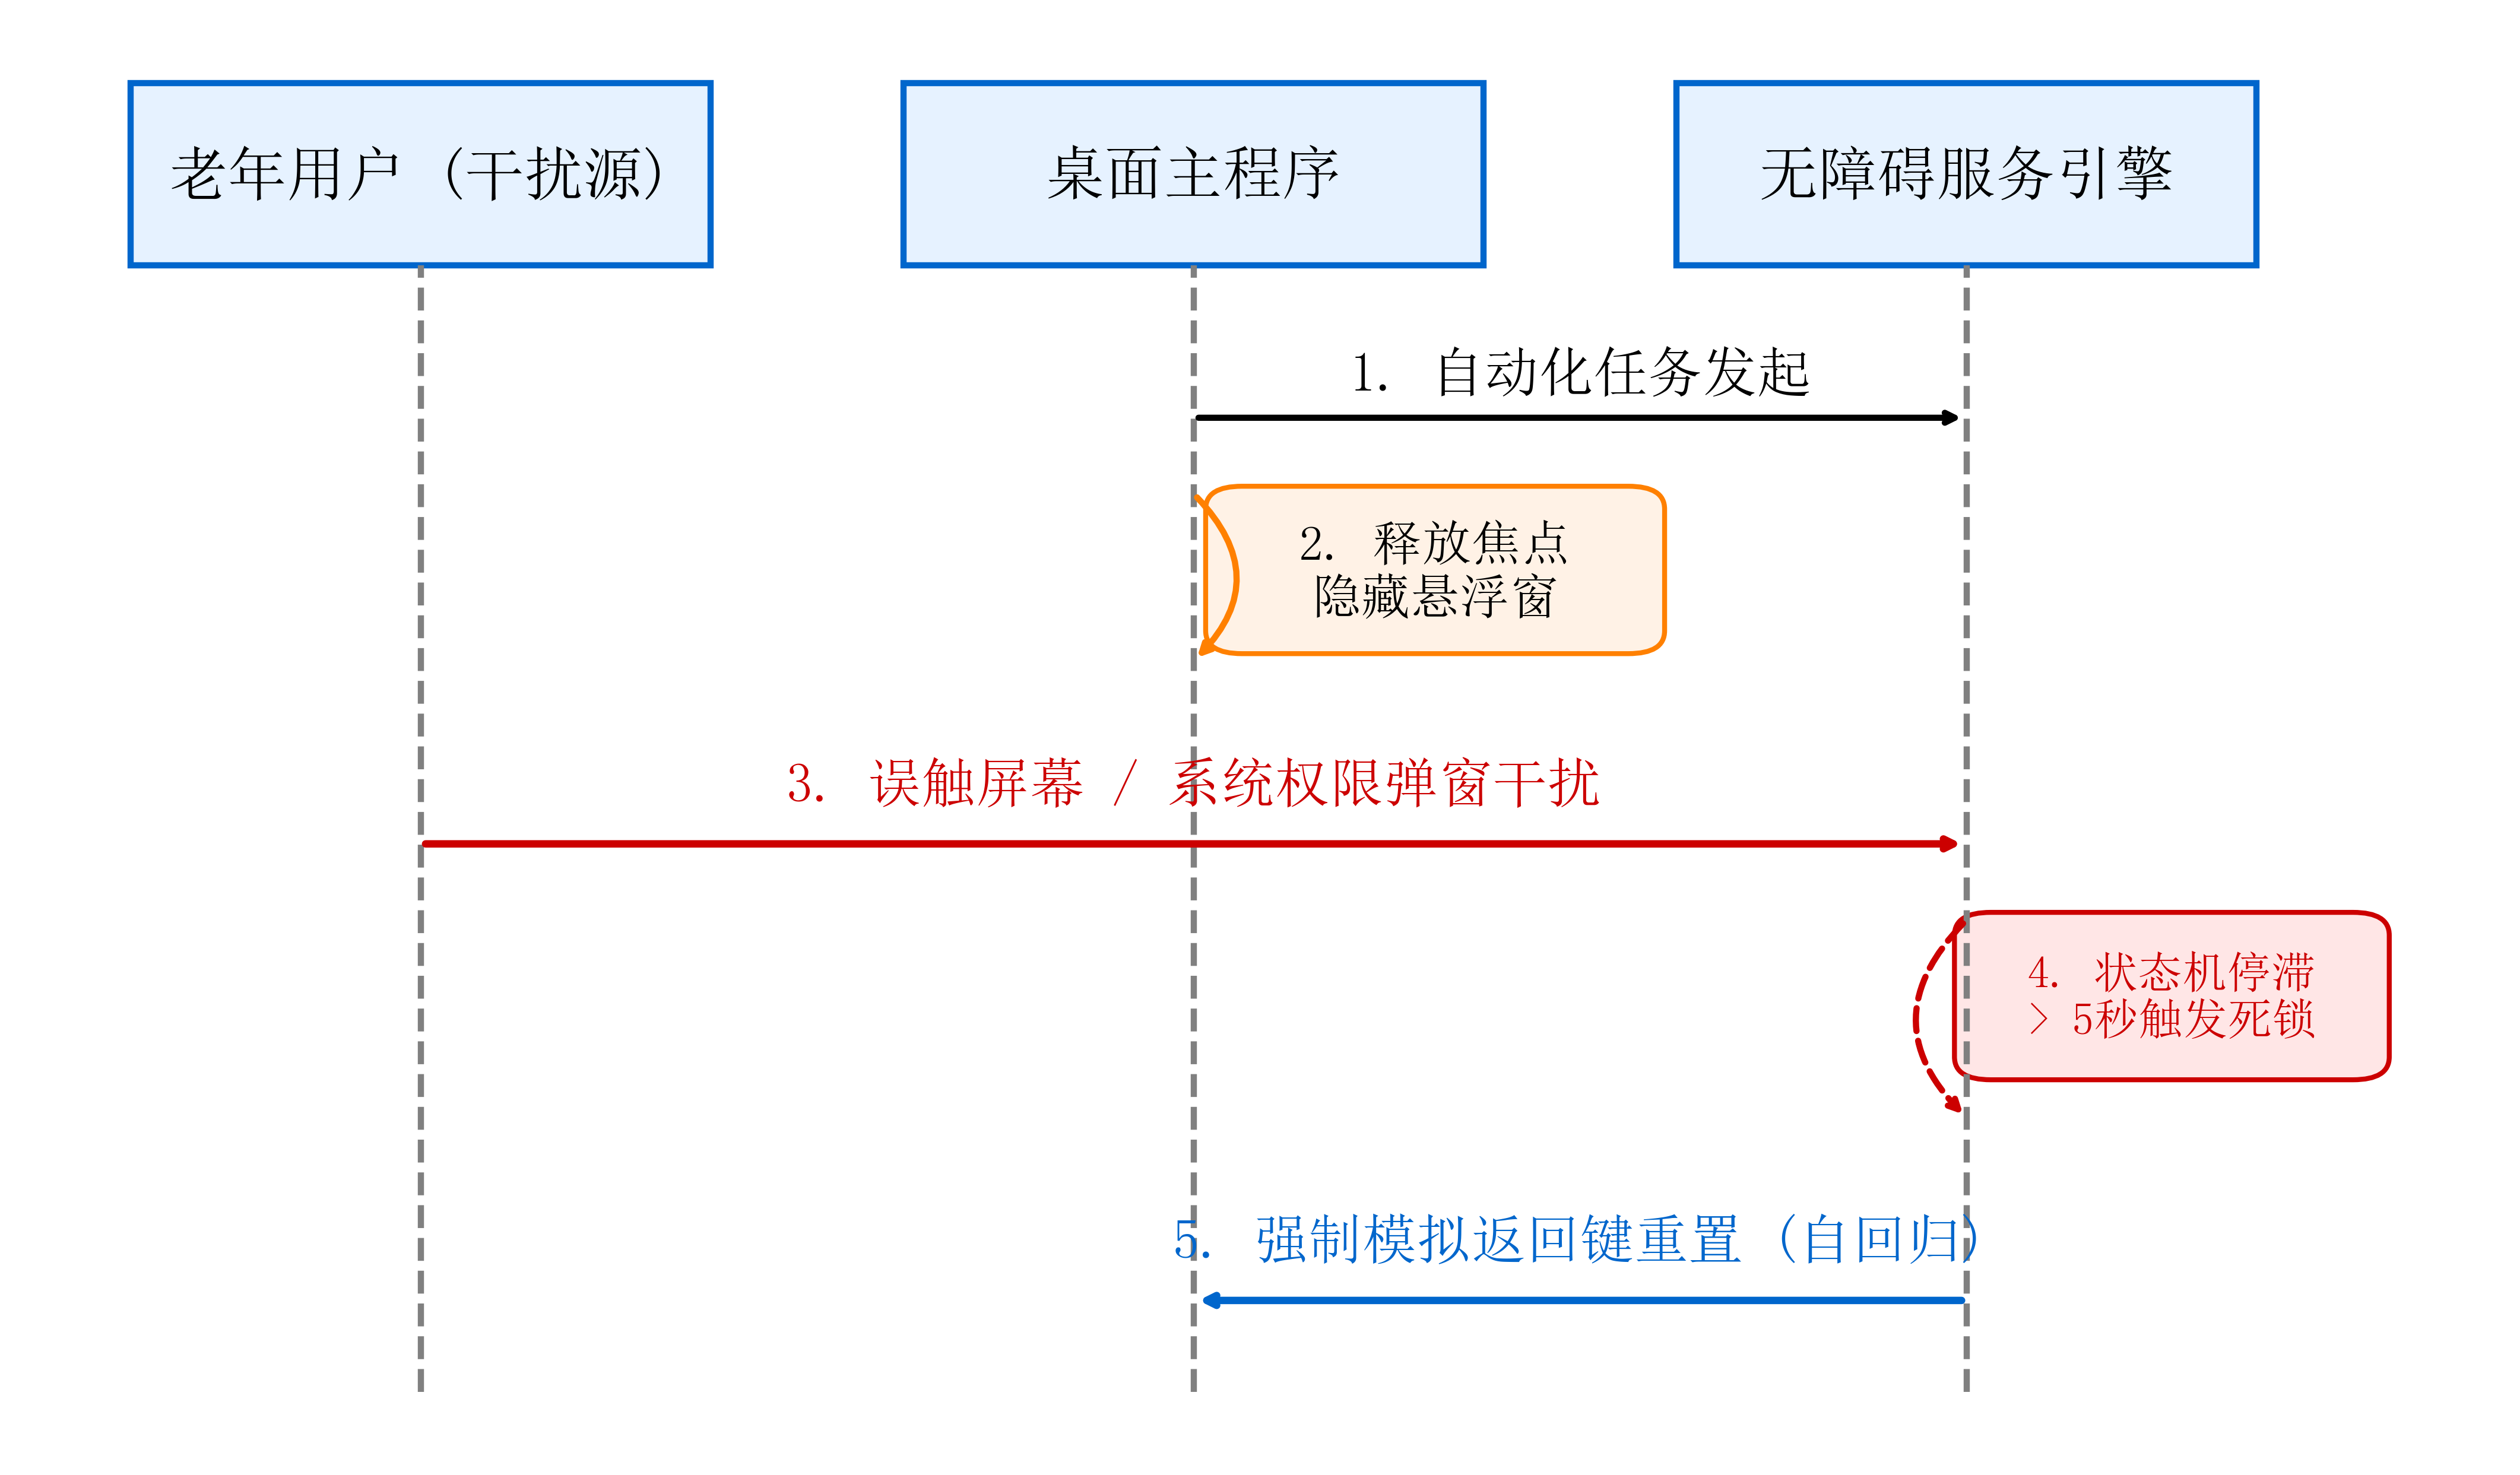
\includegraphics[width=0.85\textwidth]{figures/fig2_4_focus_retreat.png}
    \caption{面临用户误触与弹窗干扰时的焦点退避与心跳防死锁时序图}
    \label{fig:focus_retreat}
\end{figure}

\subsection{语义槽位映射与空间剪枝（Spatial Pruning）调优}

为实现在低配 SoC 设备上的流畅运行，本系统在节点检索中引入了“空间剪枝算法”。通过获取当前页面的几何边界，主动剔除 60\% 以上的非目标交互区（如系统通知栏、虚拟键盘区及无交互文本区），使 DFS（深度优先搜索）的算法复杂度从全量检索降低至目标区域检索。

同时，系统打通语音助理的语义解析（NLU）到自动化指令的映射，通过“槽位填充（Slot Filling）”技术，将“给女儿打视频”中的关键词直接映射为状态机的初始化约束条件。这种基于“语义引导、空间压缩”的协同方案，不仅提升了操作精度，更将通讯链路的建立耗时压缩至 5.4 秒左右，显著跨越了“数字鸿沟”\upcite{18}。



